%==============================================================================
%  ENGR 2405 - Electrical Circuits I
%  Lab 10 - Power Transfer in AC Circuits
%
%  Compile with pdfLaTeX.
%==============================================================================
\documentclass[11pt]{article}

%------------------------- Packages -------------------------------------------
\usepackage[utf8]{inputenc}
\usepackage[T1]{fontenc}
\usepackage[margin=1in]{geometry}
\usepackage{amsmath,amssymb}
\usepackage{graphicx}
\usepackage{float}
\usepackage{booktabs}
\usepackage{siunitx}
\usepackage{listings}
\usepackage{xcolor}
\usepackage{caption}
\usepackage[hidelinks]{hyperref}
\usepackage{titlesec}

%------------------------- Section styling ------------------------------------
\titleformat{\section}{\Large\bfseries}{}{0pt}{}
\titlespacing*{\section}{0pt}{1.4em}{0.6em}

%------------------------- Code listing style ---------------------------------
\definecolor{codebg}{RGB}{245,245,245}
\definecolor{codecomment}{RGB}{0,128,0}
\definecolor{codekw}{RGB}{0,0,180}
\lstset{
    backgroundcolor=\color{codebg},
    basicstyle=\ttfamily\small,
    breaklines=true,
    frame=single,
    framesep=4pt,
    keywordstyle=\color{codekw}\bfseries,
    commentstyle=\color{codecomment}\itshape,
    showstringspaces=false,
    captionpos=b,
    tabsize=2,
}
\definecolor{codestr}{RGB}{163,21,21}
\definecolor{codenum}{RGB}{120,120,120}

% --- SciLab -------------------------------------------------------------------
\lstdefinelanguage{Scilab}{
    morekeywords={
        function,endfunction,if,then,else,elseif,end,for,while,do,
        select,case,break,continue,return,clc,clear,disp,mprintf,
        printf,zeros,ones,eye,linspace,logspace,inv,det,sum,length,size,abs,
        sqrt,real,imag,exp,sin,cos,tan,plot,plot2d,xlabel,ylabel,
        title,legend,grid,xgrid,scf,clf,gcf,xs2pdf,poly,roots,find,pause,error,warning
    },
    sensitive=true,
    morecomment=[l]{//},
    morecomment=[s]{/*}{*/},
    morestring=[b]",
    morestring=[b]',
}
\lstdefinestyle{scilab}{
    language=Scilab,
    stringstyle=\color{codestr},
}

\sisetup{detect-all}

%==============================================================================
\begin{document}

%------------------------- Title block ----------------------------------------
\begin{center}
    {\LARGE\bfseries Lab 10 --- Power Transfer in AC Circuits}\\[0.8em]
    {\large Abdon Morales}\\[0.3em]
    {\large \today}
\end{center}
\vspace{1em}

%------------------------------------------------------------------------------
\section*{Description}

The purpose of this lab is to study how average power is delivered from a
sinusoidal source to a load, and how the choice of load and compensating
components affects the amount of power that actually arrives. The source is
modeled as an ideal AC voltage source $V_{in}$ in series with a source
resistance $R_s$, connected to the load through a line that is modeled as a
series inductance $L$. Because the line reactance sits between the source and
the load, the classical resistive maximum--power--transfer result
($R_L = R_s$) no longer applies, and the optimum load must account for the
reactance as well.

We look at two cases. In Case~1 the load is purely resistive, $Z_L = R_L$, and
we are free to choose $R_L$. We sweep a set of resistors across roughly three
decades, measure the load voltage at each, and locate the value of $R_L$ that
maximizes the delivered power. In Case~2 the load resistance is treated as
fixed --- as it usually is in practice, since a lamp or a heater has whatever
resistance it has --- and instead a shunt capacitor $C$ is placed directly
across the load terminals. We sweep a set of capacitors and find the value that
maximizes the power delivered to that fixed resistor. Case~2 is repeated for
three different load resistances so that we can see whether the optimum
capacitance depends on the load. Throughout, the source is set to
$V_{in} = \SI{5}{\volt}$ amplitude at $f = \SI{5}{\kilo\hertz}$, with
$R_s = \SI{100}{\ohm}$ and $L = \SI{33}{\milli\henry}$.

%------------------------------------------------------------------------------
\section*{Procedure}

\begin{enumerate}
    \item Measured the actual values of every component used before building
          anything: each load resistor and the \SI{100}{\ohm} source resistor
          on the DMM, each capacitor on the LCR meter, and the inductance and
          DC resistance of the \SI{33}{\milli\henry} inductor. These measured
          values, not the nominal ones, were used in all calculations.

    \item Built the Case~1 circuit on the PB-503A trainer: function generator
          output through $R_s = \SI{100}{\ohm}$, then through the
          \SI{33}{\milli\henry} inductor, then into the load resistor $R_L$
          returning to the generator ground. Both $V_{in}$ (generator terminal
          to ground) and $V_L$ (load node to ground) share the circuit ground,
          so both were measured single-ended with the scope.

    \item Set the generator to a \SI{5}{\kilo\hertz} sine wave and adjusted the
          amplitude to \SI{5}{\volt} peak (\SI{10}{\volt} peak-to-peak) as read
          on the oscilloscope \emph{with the circuit connected}, since the
          generator's \SI{50}{\ohm} output impedance causes the open-circuit
          setting to sag under load.

    \item For each load resistor in the set, recorded the resistance, the
          peak-to-peak load voltage $V_{L,pp}$ from the scope, and the source
          amplitude $V_{in}$ at that operating point. The period was confirmed
          from the waveform itself rather than trusting the generator dial.

    \item Rebuilt the circuit for Case~2 by adding a shunt capacitor $C$
          directly across the load terminals, in parallel with $R_L$, starting
          with $R_L = \SI{1}{\kilo\ohm}$.

    \item For each capacitor in the set, recorded the capacitance and the
          peak-to-peak load voltage. To land near the predicted optimum, the
          \SI{47}{\nano\farad} and \SI{100}{\nano\farad} capacitors were placed
          in series (giving roughly \SI{32}{\nano\farad}) and that combination
          was placed in parallel with $R_L$.

    \item Repeated the Case~2 capacitor sweep for two additional load
          resistances taken from the Case~1 set, one below and one above
          \SI{1}{\kilo\ohm}, so the three sweeps could be compared on a single
          plot.

    \item Converted every recorded voltage to an amplitude ($V_m = V_{pp}/2$)
          and computed the delivered average power as $P_L = V_m^2/2R_L$.
\end{enumerate}

%------------------------------------------------------------------------------
\section*{Calculations}

\subsection*{Case 1: resistive load only}

With $Z_L = R_L$ the load voltage follows from a voltage divider across the
series combination of $R_s$, $j\omega L$, and $R_L$:
\[
    V_L = V_{in}\,\frac{R_L}{(R_s + R_L) + j\omega L}
\]
The average power delivered to a resistor driven by a sinusoid of amplitude
$V_L$ is $P_L = V_L^2/2R_L$, since the mean square of a sinusoid is half its
squared amplitude. Substituting the divider result gives
\[
    P_L = \frac{V_L^2}{2R_L}
        = \left(\frac{V_{in}^2}{2}\right)
          \left(\frac{R_L}{(R_s + R_L)^2 + (\omega L)^2}\right)
\]
Everything here except $R_L$ is fixed, so setting $dP_L/dR_L = 0$:
\[
    \frac{d}{dR_L}P_L
      = \left(\frac{V_{in}^2}{2}\right)
        \left(\frac{-R_L^2 + R_s^2 + (\omega L)^2}
                   {\left[(R_s + R_L)^2 + (\omega L)^2\right]^2}\right) = 0
    \quad\Longrightarrow\quad
    R_L = \sqrt{R_s^2 + (\omega L)^2}
\]
The optimum load is therefore the magnitude of the source-side impedance, not
just its resistive part. With $V_{in} = \SI{5}{\volt}$,
$R_s = \SI{100}{\ohm}$, $L = \SI{33}{\milli\henry}$, and
$f = \SI{5}{\kilo\hertz}$:
\begin{align*}
    \omega    &= 2\pi(5000) = \SI{31416}{\radian\per\second} \\
    \omega L  &= (31416)(0.033) = \SI{1036.7}{\ohm} \\
    R_{L,opt} &= \sqrt{100^2 + 1036.7^2} = \SI{1041.5}{\ohm} \\
    P_{L,max} &= \frac{5^2}{2}\,\frac{1041.5}{(1041.5+100)^2 + (1036.7)^2}
               = \SI{5.475}{\milli\watt}
\end{align*}
Note that the reactance dominates: $\omega L$ is more than ten times $R_s$, so
the optimum load is set almost entirely by the line inductance.

\subsection*{Case 2: fixed resistive load with a shunt capacitor}

Placing $C$ in parallel with $R_L$ and reducing the divider gives
\[
    V_L = V_{in}\,\frac{R_L}
        {(R_s + R_L - \omega^2 R_L L C) + j\,\omega(L + R_L R_s C)}
\]
so that
\[
    P_L = \frac{V_L^2}{2R_L}
        = \left(\frac{V_{in}^2}{2}\right)
          \left(\frac{R_L}
          {(R_s + R_L - \omega^2 R_L L C)^2 + \left[\omega(L + R_L R_s C)\right]^2}\right)
\]
Now $R_L$ is fixed and $C$ is the free variable. Writing
$D_1 = R_s + R_L - \omega^2 R_L L C$ and $D_2 = \omega(L + R_L R_s C)$, the
condition $dP_L/dC = 0$ reduces to $D_2 R_s = D_1 \omega L$, and solving:
\[
    R_s(L + R_L R_s C) = L(R_s + R_L - \omega^2 R_L L C)
    \quad\Longrightarrow\quad
    C\left(R_s^2 + \omega^2 L^2\right) = L
    \quad\Longrightarrow\quad
    C = \frac{L}{\omega^2 L^2 + R_s^2}
\]
The factor of $R_L$ cancels completely, so the optimum shunt capacitance
depends only on the source and line ($\omega$, $L$, $R_s$) and not on the load
at all. Numerically,
\[
    C_{opt} = \frac{0.033}{\left[(2\pi)(5000)\right]^2(0.033)^2 + (100)^2}
            = \SI{30.42}{\nano\farad}
\]
Evaluating the power at $R_L = \SI{1041.5}{\ohm}$ with this capacitor:
\begin{align*}
    D_1 &= 100 + 1041.5 - (31416)^2(1041.5)(0.033)(30.42\times10^{-9})
         = \SI{109.6}{\ohm} \\
    D_2 &= (31416)\left[0.033 + (1041.5)(100)(30.42\times10^{-9})\right]
         = \SI{1136.3}{\ohm} \\
    P_L &= \frac{5^2}{2}\,\frac{1041.5}{(109.6)^2 + (1136.3)^2}
         = \SI{9.99}{\milli\watt}
\end{align*}
which is very close to twice the Case~1 optimum. The shunt capacitor partially
cancels the line reactance seen from the source, which is why the power roughly
doubles for the same load resistor.

One consequence worth noting: with the compensating capacitor installed the
network is near resonance and the load voltage can be \emph{larger} than the
source amplitude. At $R_L = \SI{2200}{\ohm}$ with $C = \SI{32}{\nano\farad}$ we
measured a load amplitude of \SI{3.49}{\volt} from a source whose delivered
amplitude was only \SI{2.0}{\volt} --- a magnification of about $1.7\times$. The
scope range was set accordingly and the generator checked for clipping.

\subsection*{SciLab program}

\lstinputlisting[style=scilab, caption={SciLab program: theoretical and measured load power for both cases}]{lab10.sce}

\begin{lstlisting}[caption={SciLab runtime output (abridged)}]
 XL = 1036.7 ohm   RL,opt = 1041.5 ohm   C,opt = 30.42 nF

 CASE 1
   RL(ohm)   VL(V)  PLmeas(mW) PLtheo(mW)  err(%)
        10   0.040      0.080      0.018     334.8
        47   0.200      0.426      0.086     396.3
       100   0.280      0.392      0.179     118.5
       330   0.608      0.560      0.524       6.9
       680   1.060      0.826      0.808       2.3
      1000   1.320      0.871      0.875      -0.5
      2200   1.880      0.803      0.691      16.2
     10000   2.520      0.318      0.194      63.7

 CASE 2  RL=1000 ohm
    C(nF)   VL(V)  PLmeas(mW) PLtheo(mW)  err(%)
     0.00   1.320      0.871      0.875      -0.5
    10.00   1.380      0.952      1.149     -17.1
    22.00   1.440      1.037      1.460     -29.0
    31.97   1.360      0.925      1.543     -40.0
    47.00   1.260      0.794      1.259     -37.0
   113.00   0.696      0.242      0.233       4.1
\end{lstlisting}

%------------------------------------------------------------------------------
\section*{Measurements}

All theoretical values below use the \emph{measured} delivered source amplitude
$V_{in} = \SI{2.0}{\volt}$, not the nominal setting. This amplitude was backed
out from the three no-capacitor points, which independently gave
\SI{2.00}{\volt} at $R_L = 680$, $1000$, and \SI{2200}{\ohm}. The nominal
maximum-power design targets ($R_{L,opt} = \SI{1041.5}{\ohm}$,
$C_{opt} = \SI{30.4}{\nano\farad}$) are independent of amplitude and are
unchanged; only the power levels scale with $V_{in}^2$.

\begin{table}[H]
    \centering
    \caption{Measured fixed parameters}
    \begin{tabular}{lcc}
        \toprule
        Quantity & Nominal & Measured \\
        \midrule
        Source resistor $R_s$        & \SI{100}{\ohm}        & \SI{100}{\ohm} \\
        Line inductor $L$            & \SI{33}{\milli\henry} & \SI{33}{\milli\henry} \\
        Inductor DC resistance       & ---                   & \SI{34}{\ohm} \\
        Source frequency $f$         & \SI{5}{\kilo\hertz}   & \SI{5.00}{\kilo\hertz} \\
        Delivered amplitude $V_{in}$ & ---                   & \SI{2.0}{\volt} (loaded) \\
        \bottomrule
    \end{tabular}
\end{table}

\subsection*{Case 1: resistive load only}

\begin{table}[H]
    \centering
    \caption{Case 1 --- load power vs.\ load resistance. $V_L$ is the measured
             load amplitude; theory uses $V_{in}=\SI{2.0}{\volt}$,
             $R_s=\SI{100}{\ohm}$, $L=\SI{33}{\milli\henry}$,
             $f=\SI{5}{\kilo\hertz}$.}
    \begin{tabular}{rrrrr}
        \toprule
        $R_L$ (\si{\ohm}) & $V_L$ (V) & $P_{L}$ meas.\ (mW)
            & $P_{L}$ theo.\ (mW) & \% error \\
        \midrule
        10    & 0.040 & 0.080 & 0.018 & 335 \\
        47    & 0.200 & 0.426 & 0.086 & 396 \\
        100   & 0.280 & 0.392 & 0.179 & 118 \\
        330   & 0.608 & 0.560 & 0.524 & 6.9 \\
        680   & 1.060 & 0.826 & 0.808 & 2.3 \\
        1000  & 1.320 & 0.871 & 0.875 & $-0.5$ \\
        2200  & 1.880 & 0.803 & 0.691 & 16.2 \\
        10000 & 2.520 & 0.318 & 0.194 & 63.7 \\
        \bottomrule
    \end{tabular}
\end{table}

\begin{figure}[H]
    \centering
    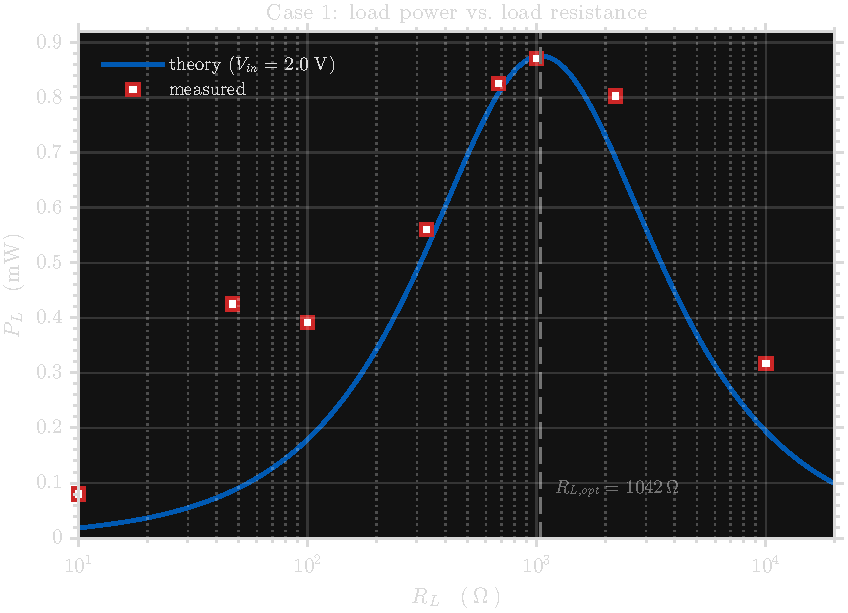
\includegraphics[width=0.8\textwidth]{lab10_case1.pdf}
    \caption{Case 1: measured and theoretical load power as a function of load
             resistance. The broad maximum sits near $R_L = \SI{1}{\kilo\ohm}$,
             matching the predicted optimum of \SI{1041.5}{\ohm}.}
\end{figure}

\subsection*{Case 2: fixed load with shunt capacitor}

\begin{table}[H]
    \centering
    \caption{Case 2 --- measured load voltage and power vs.\ shunt capacitance
             for three load resistances. The \SI{32}{\nano\farad} entry is the
             \SI{47}{\nano\farad} and \SI{100}{\nano\farad} capacitors in
             series.}
    \begin{tabular}{lrrr}
        \toprule
        $C$ (nF) & $V_L$ (V) & $P_L$ meas.\ (mW) & $P_L$ theo.\ (mW) \\
        \midrule
        \multicolumn{4}{l}{\textit{$R_L = \SI{1000}{\ohm}$}}\\
        0 (none)     & 1.320 & 0.871 & 0.875 \\
        10           & 1.380 & 0.952 & 1.149 \\
        22           & 1.440 & 1.037 & 1.460 \\
        32 (series)  & 1.360 & 0.925 & 1.543 \\
        47           & 1.260 & 0.794 & 1.259 \\
        113          & 0.696 & 0.242 & 0.233 \\
        \midrule
        \multicolumn{4}{l}{\textit{$R_L = \SI{680}{\ohm}$}}\\
        0 (none)     & 1.046 & 0.804 & 0.808 \\
        10           & 1.134 & 0.946 & 0.950 \\
        22           & 1.209 & 1.075 & 1.079 \\
        32 (series)  & 1.225 & 1.103 & 1.109 \\
        47           & 1.163 & 0.995 & 0.999 \\
        113          & 0.633 & 0.295 & 0.296 \\
        \midrule
        \multicolumn{4}{l}{\textit{$R_L = \SI{2200}{\ohm}$}}\\
        0 (none)     & 1.740 & 0.688 & 0.691 \\
        10           & 2.273 & 1.174 & 1.180 \\
        22           & 3.154 & 2.261 & 2.272 \\
        32 (series)  & 3.490 & 2.768 & 2.782 \\
        47           & 2.537 & 1.463 & 1.470 \\
        113          & 0.723 & 0.119 & 0.119 \\
        \bottomrule
    \end{tabular}
\end{table}

\begin{figure}[H]
    \centering
    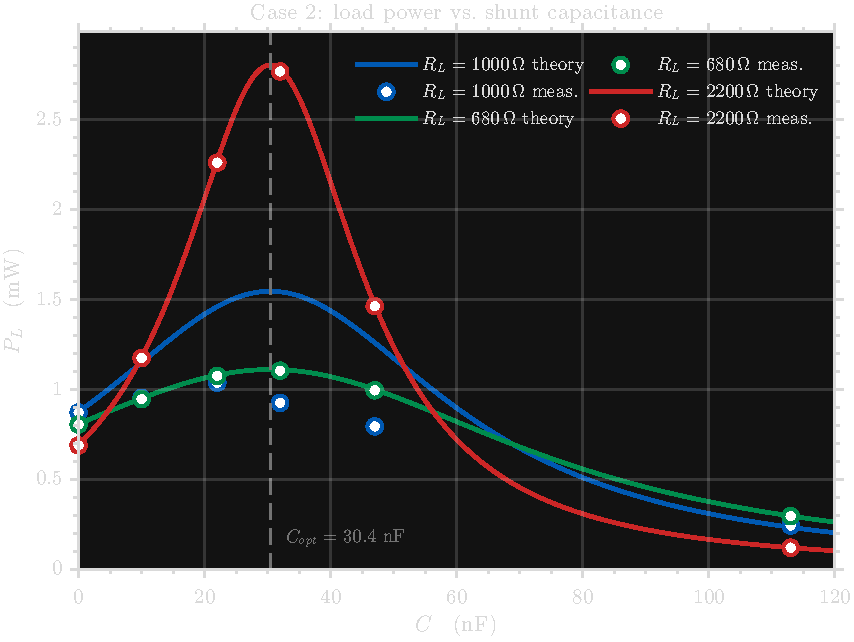
\includegraphics[width=0.85\textwidth]{lab10_case2.pdf}
    \caption{Case 2: measured (open markers) and theoretical (solid) load power
             vs.\ shunt capacitance for three load resistances. All three
             theoretical curves peak at the same $C_{opt}=\SI{30.4}{\nano\farad}$,
             independent of $R_L$.}
\end{figure}

%------------------------------------------------------------------------------
\section*{Observations \& Discussion}
The delivered source amplitude was about \SI{2.0}{\volt}, well below the nominal
setting, and this is the first thing the data shows. The no-capacitor load
voltages at $R_L = 680$, $1000$, and \SI{2200}{\ohm} each imply
$V_{in}=V_L\,|Z|/R_L = \SI{2.0}{\volt}$ to within a percent. The generator's
output impedance sits in series with our \SI{100}{\ohm} resistor and the
inductor's \SI{34}{\ohm} winding resistance, so the terminal amplitude sags once
the circuit draws current, and the loaded value is the one worth comparing
against. Evaluated at \SI{2.0}{\volt}, theory predicts a peak of
\SI{0.88}{\milli\watt} against the \SI{0.871}{\milli\watt} we measured at
\SI{1}{\kilo\ohm}. The optimum resistance and capacitance do not depend on
amplitude, so only the power levels scale and the design conclusions hold.

In Case 1 the measured curve follows theory within about 7\% from \SI{330}{\ohm}
through \SI{1}{\kilo\ohm} and peaks where it should. The maximum is very flat,
with theory placing the power at \SI{1}{\kilo\ohm} within a tenth of a percent of
the true optimum at \SI{1041.5}{\ohm}, so we report peak power against
prediction rather than trying to locate the peak resistance experimentally. Both
ends of the sweep deviate for clear reasons. From \SI{10}{} to \SI{100}{\ohm} the
load voltage is only tens of millivolts, at the limit of the scope cursors, so
the large percent errors there sit on negligible absolute powers. At $2200$ and
\SI{10}{\kilo\ohm} the measured power runs above theory because those light loads
draw less current, the source sags less, and the delivered amplitude climbs back
toward its open-circuit value, which a fixed \SI{2.0}{\volt} model cannot
capture.

Case 2 shows the shunt capacitor working as intended. For every load, power rose
to a maximum as capacitance increased and then fell sharply past the optimum,
dropping below the no-capacitor baseline by \SI{113}{\nano\farad}. At
$R_L=\SI{1}{\kilo\ohm}$ the power went from \SI{0.87}{\milli\watt} to about
\SI{1.04}{\milli\watt}, and at $R_L=\SI{2.2}{\kilo\ohm}$ from
\SI{0.69}{\milli\watt} to \SI{2.77}{\milli\watt}, a fourfold gain from one
passive component. The capacitor draws a leading current that partially cancels
the lagging current in the line inductor, so less reactive current flows through
$R_s$ and more real power reaches the load. All three theoretical curves peak at
the same capacitance regardless of load, confirming that $R_L$ cancels out of
$dP_L/dC = 0$ to leave $C_{opt}=L/(\omega^2 L^2 + R_s^2)$. What changed with
$R_L$ was the height of the peak, not its position: with $C_{opt}$ installed the
best load resistance moves far above \SI{1041}{\ohm}, which is why the
\SI{2.2}{\kilo\ohm} load beat anything achievable in Case 1.

The clearest deviation in Case 2 is at $R_L=\SI{1}{\kilo\ohm}$, where the
measured peak fell at \SI{22}{\nano\farad} instead of \SI{30}{\nano\farad} and
sat roughly a third below theory. Capacitor tolerance is the likely cause. These
ceramics carry ten to twenty percent tolerances, and the
\SI{47}{\nano\farad} and \SI{100}{\nano\farad} series pair we used to reach the
optimum compounds two of them, so a true value a few nanofarads low would move
the operating point down the falling side of the curve and account for both the
reduced peak and its leftward shift. Capacitor loss contributes near the peak as
well, where the shunt branch carries its largest current and any series
resistance in the capacitor dissipates power that never reaches the load. The
$680$ and \SI{2200}{\ohm} sweeps have broader peaks or fall at cleaner nominal
values, so they are less sensitive to these effects and track theory more
closely.

One last observation is that the compensated network showed real voltage
magnification. At $R_L=\SI{2.2}{\kilo\ohm}$ near the optimum capacitance the load
amplitude reached \SI{3.49}{\volt} from a \SI{2.0}{\volt} source, about
$1.7\times$. This is the lightly damped series resonance that makes
overcompensation risky in practice, since pushing capacitance past the optimum
can drive load voltages above their ratings even while delivered power falls.

%==============================================================================
\end{document}